\subsection{Bilder zur Amplitudenmodulation}

\begin{figure}[H]
	\centering
	\begin{subfigure}[c]{\textwidth}
		\centering
		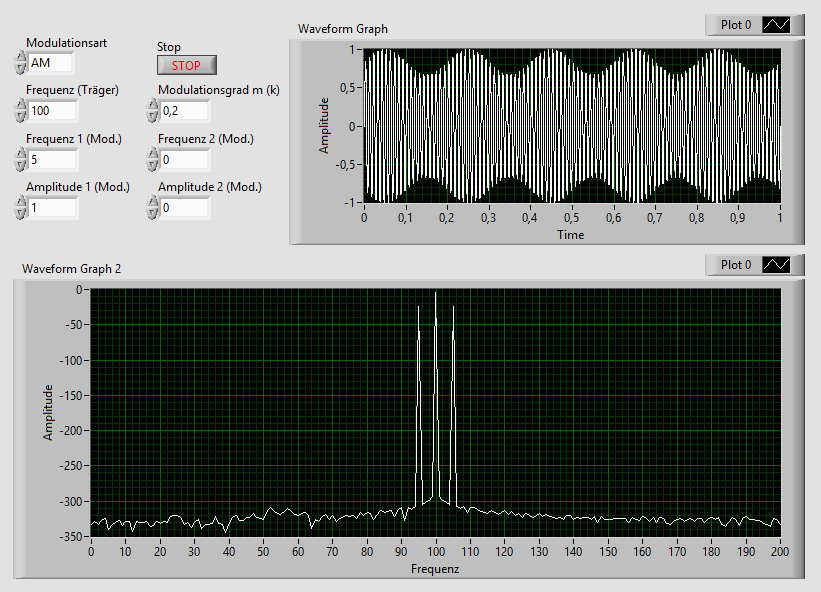
\includegraphics[width=0.7\textwidth]{pic/am_anhang_1.png}
		\subcaption{Modulation mit Trägerfrequenz 100Hz, Mod. Frequenz 5Hz, Mod. Amplitude 1, Modulationsgrad 0,2.}
	\end{subfigure}
	\begin{subfigure}[c]{\textwidth}
		\centering
		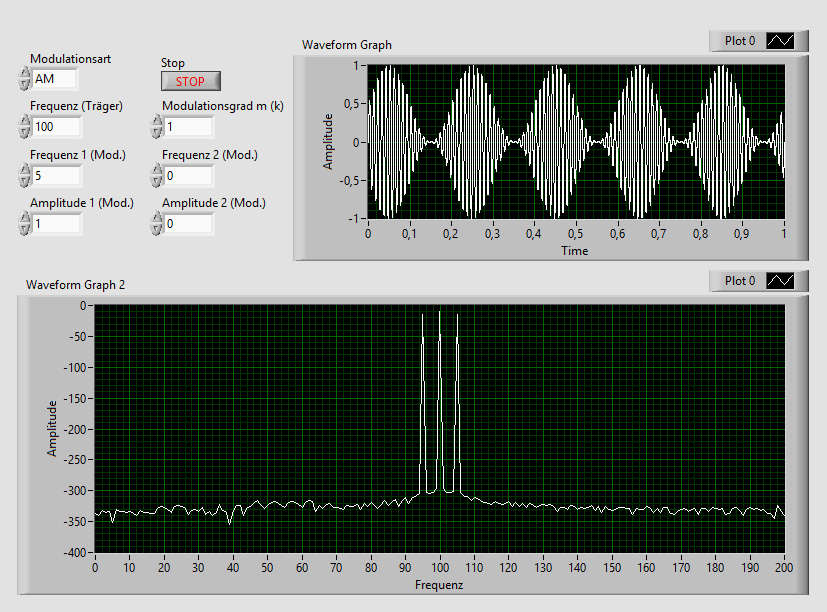
\includegraphics[width=0.7\textwidth]{pic/am_anhang_2.png}
		\subcaption{Modulation mit Trägerfrequenz 100Hz, Mod. Frequenz 5Hz, Mod. Amplitude 1, Modulationsgrad 1.}
	\end{subfigure}	
	\caption{Zwei zusätzliche Beispiele zur Amplitudenmodulation.}
	\label{fig:a1}	
\end{figure}

\subsection{Bilder zur Demodulation von Amplitudenmodulierten Signalen}

\begin{figure}[H]
	\centering
	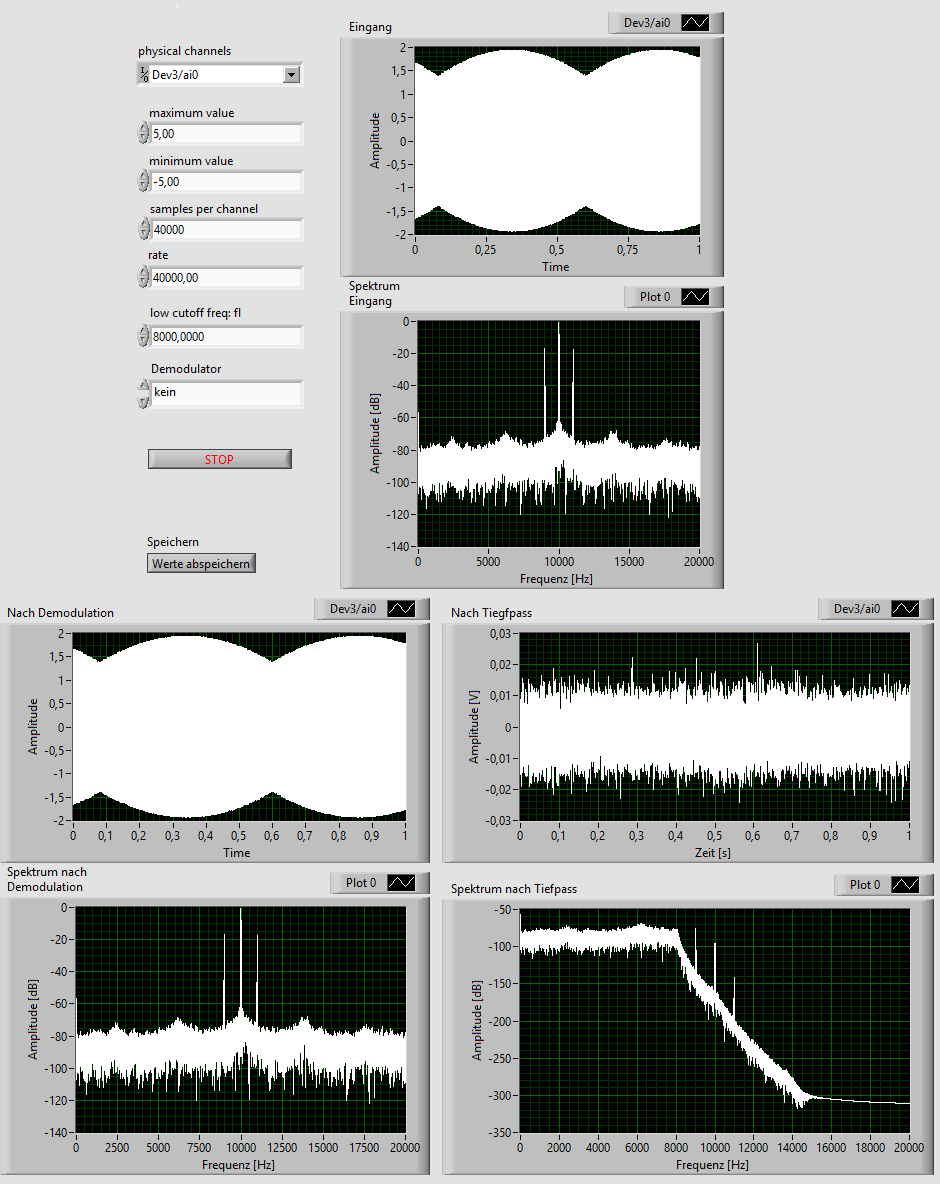
\includegraphics[width=0.9\textwidth]{pic/dam_2_keine.png}
	\caption{Testsignal 2, kein Demodulator.}
	\label{fig:a2}	
\end{figure} 

\newpage

\begin{figure}[H]
	\centering
	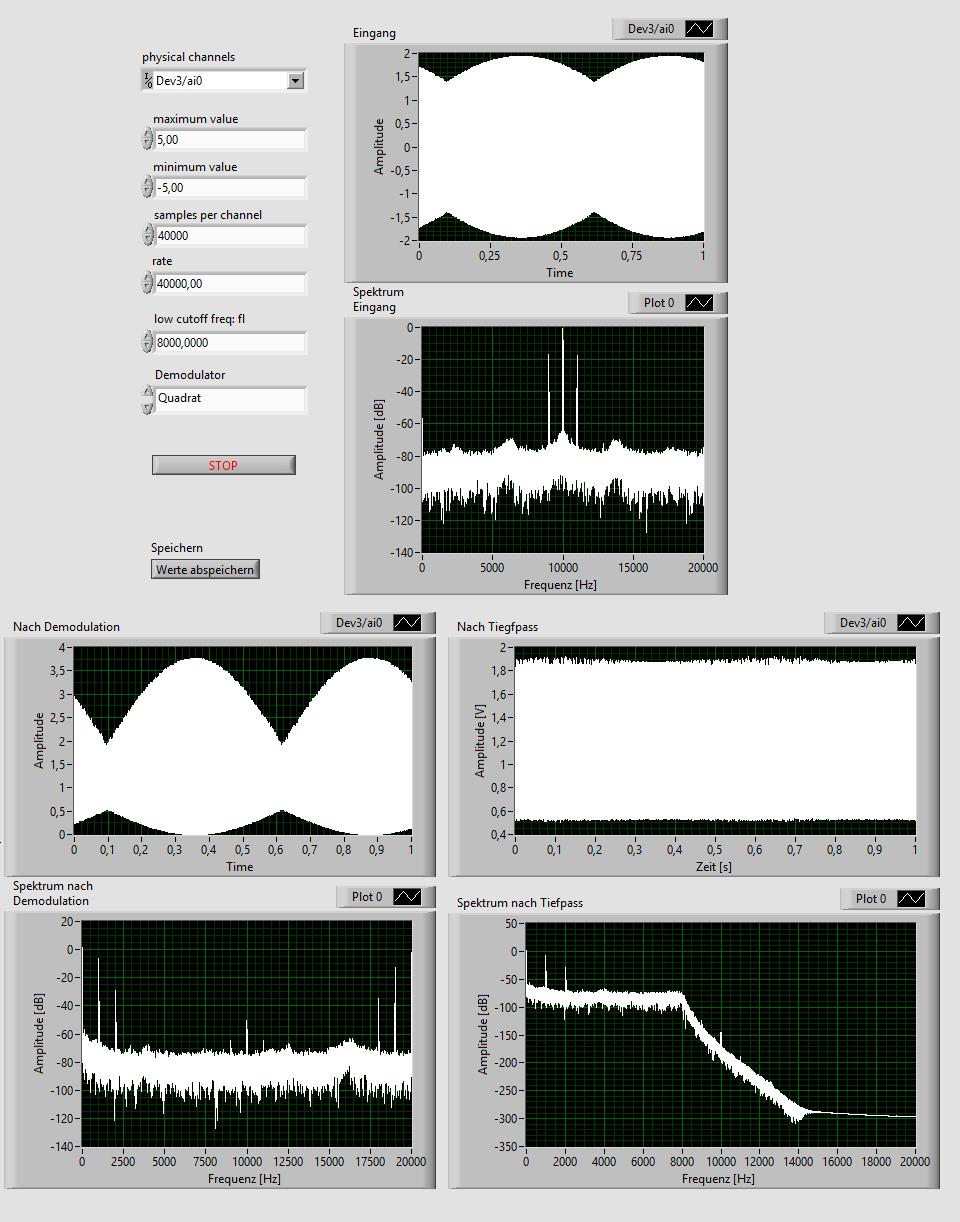
\includegraphics[width=0.9\textwidth]{pic/dam_2_quadrat.png}
	\caption{Testsignal 2, Quadrat. Demodulator.}
	\label{fig:a3}	
\end{figure}

\newpage

\begin{figure}[H]
	\centering
	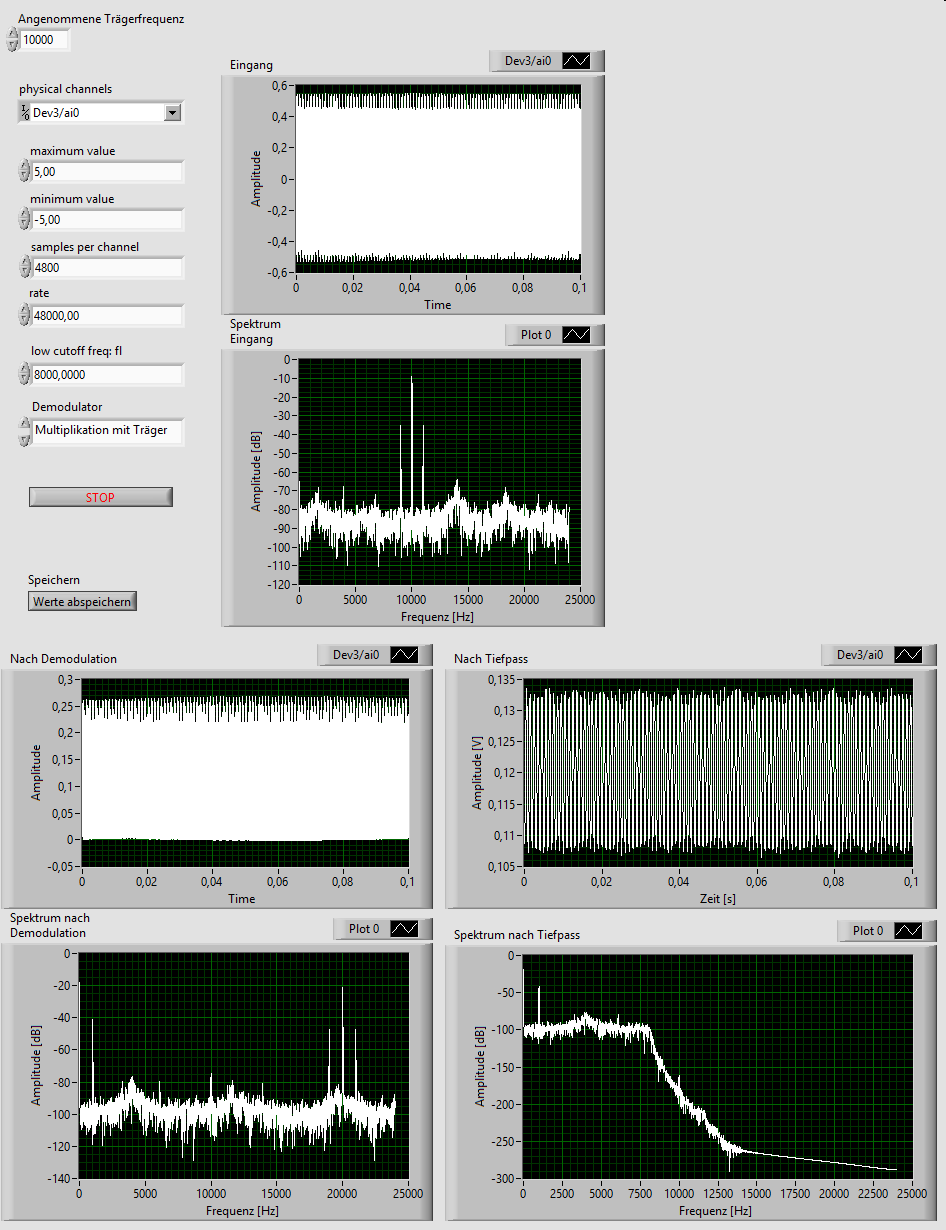
\includegraphics[width=0.9\textwidth]{pic/dam_3_traeger.png}
	\caption{Testsignal 3, Träger. Demodulator.}
	\label{fig:a4}	
\end{figure}

\newpage

\begin{figure}[H]
	\centering
	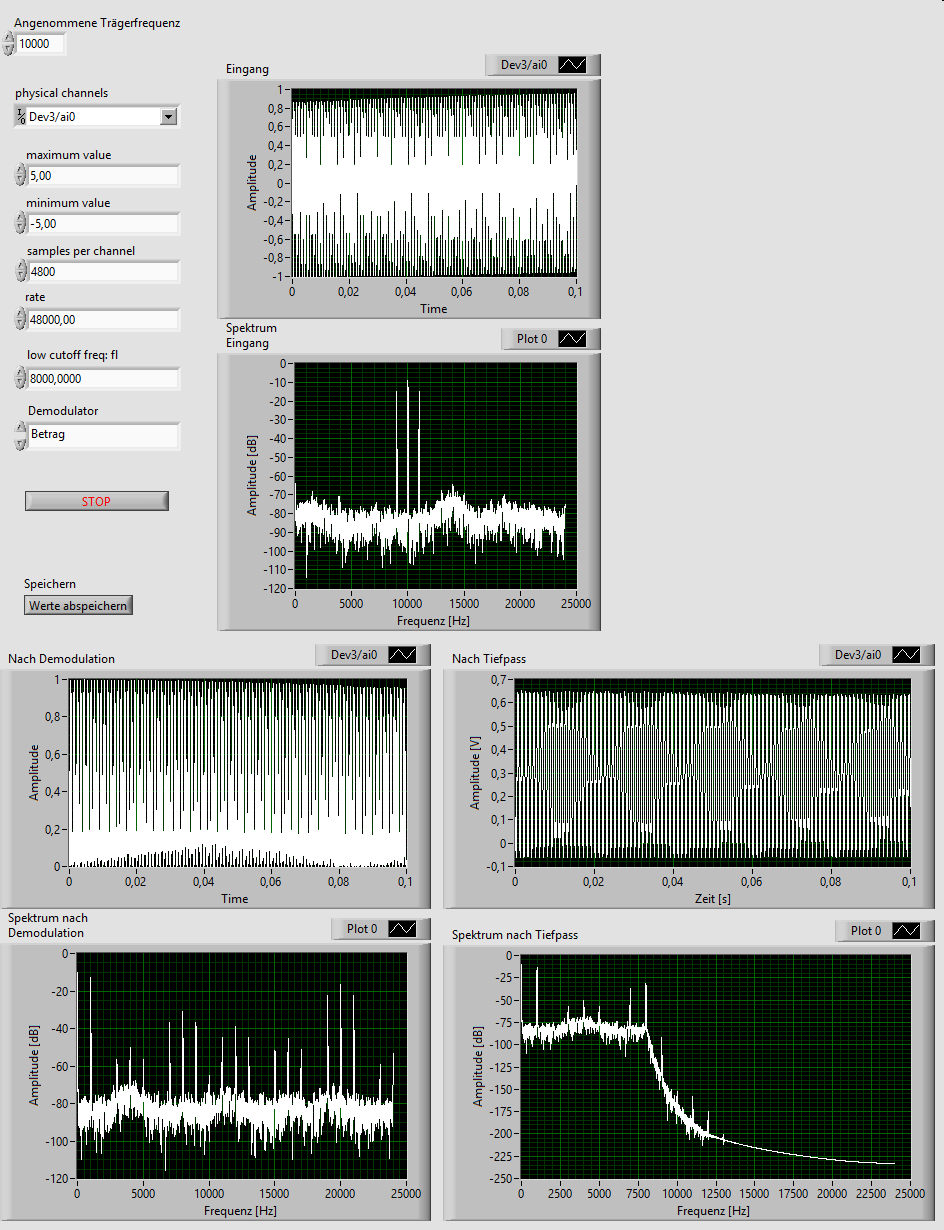
\includegraphics[width=0.9\textwidth]{pic/dam_4_betrag.png}
	\caption{Testsignal 4, Betrag. Demodulator.}
	\label{fig:a5}	
\end{figure}

\newpage

\begin{figure}[H]
	\centering
	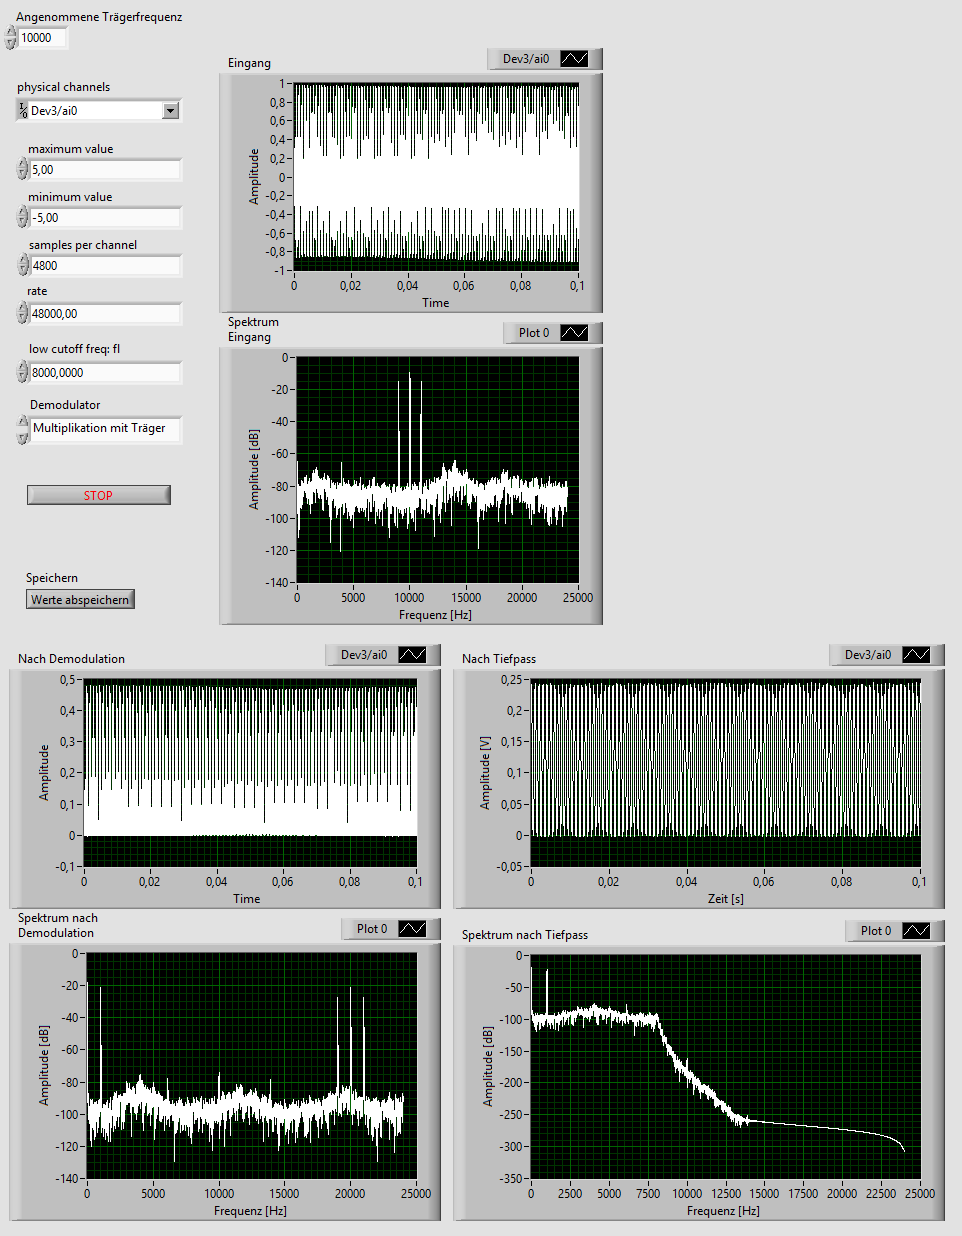
\includegraphics[width=0.9\textwidth]{pic/dam_4_traeger.png}
	\caption{Testsignal 4, Träger. Demodulator.}
	\label{fig:a6}	
\end{figure}

\newpage

\subsection{Bilder zur Frequenzmodulation}

\begin{figure}[H]
	\centering
	\begin{subfigure}[c]{\textwidth}
		\centering
		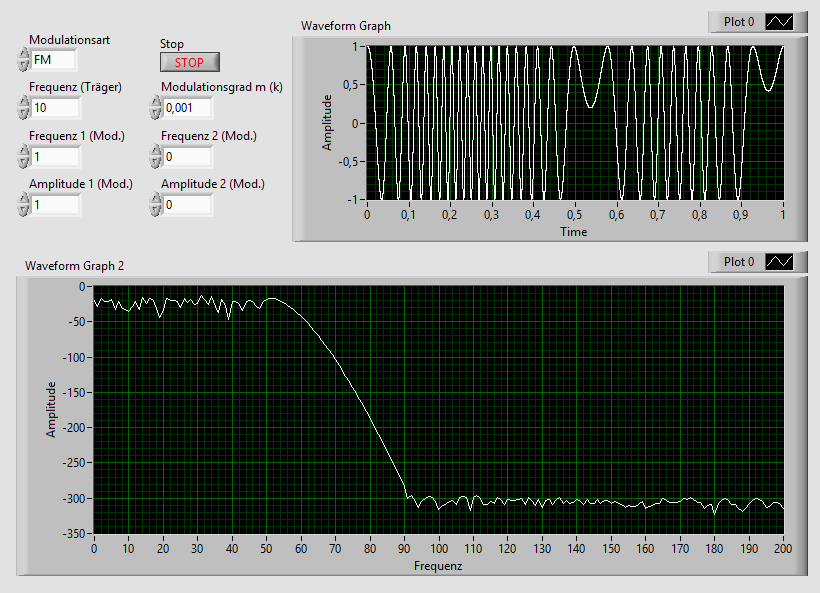
\includegraphics[width=0.7\textwidth]{pic/fmt10.png}
		\subcaption{Trägerfrequenz 10 Hz, Mod. Frequenz 1 Hz, Mod. Amplitude 1, Modulationsgrad 0,001.}
	\end{subfigure}
	\begin{subfigure}[c]{\textwidth}
		\centering
		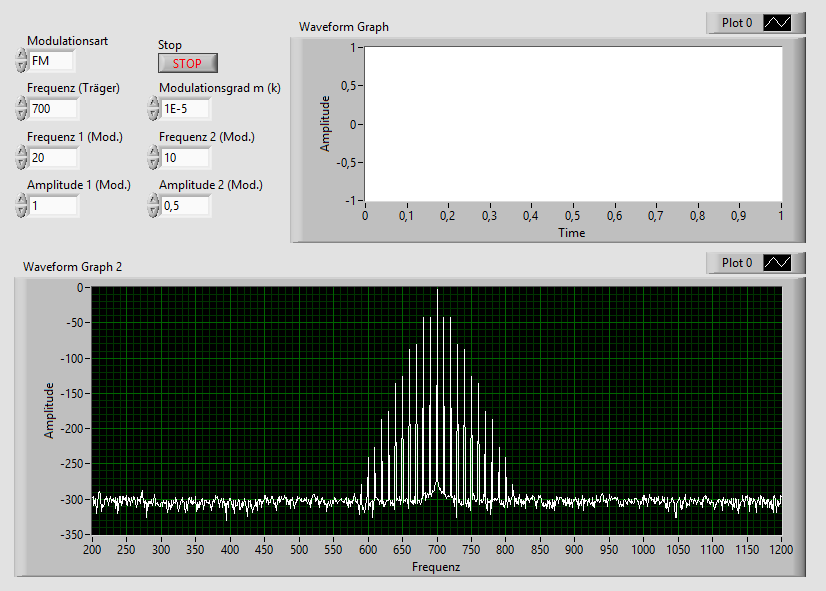
\includegraphics[width=0.7\textwidth]{pic/fmt700.png}
		\subcaption{Trägerfrequenz 700 Hz, Mod. Frequenz 10 Hz und 20 Hz, Mod. Amplitude 0,5 und 1, Modulationsgrad $10^{-5}$.}
	\end{subfigure}	
	\caption{Zwei zusätzliche Beispiele zur Frequenzmodulation.}
	\label{fig:a7}	
\end{figure}


\newpage

\subsection{Bilder zur Phasenmodulation}

\begin{figure}[H]
	\centering
	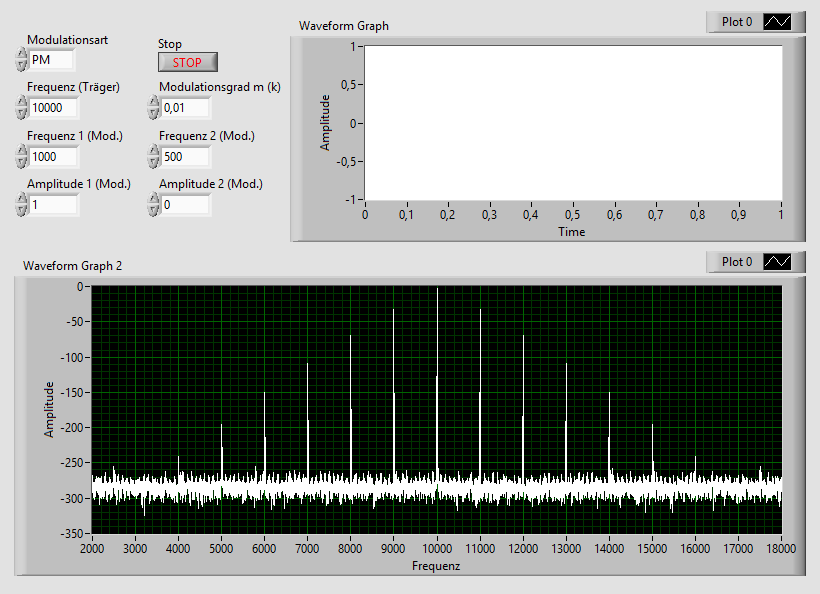
\includegraphics[width=0.7\textwidth]{pic/t10km1kg001.png}
	\caption{Weiteres Beispiel zur Phasenmodulation. Die Parameter können der Abbildung entnommen werden.}
	\label{fig:a8}	
\end{figure} 

\begin{figure}[H]
	\centering
	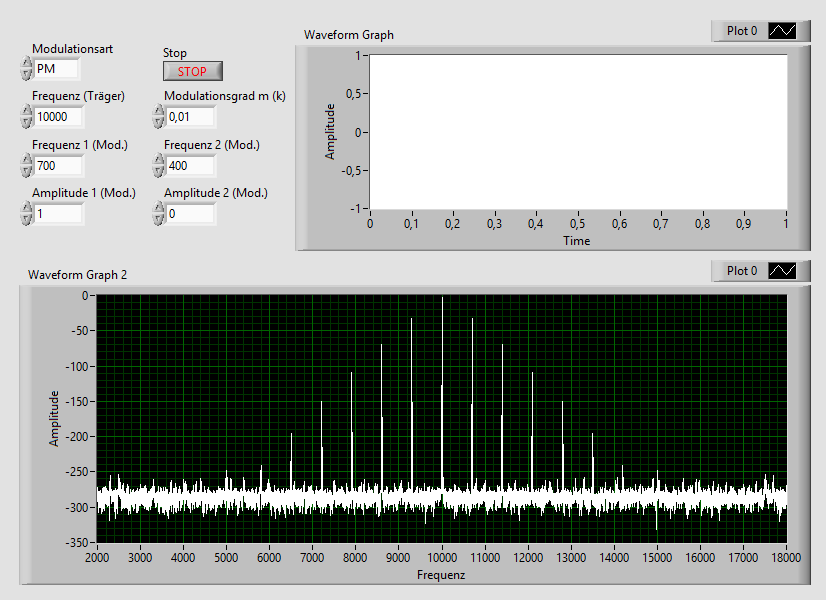
\includegraphics[width=0.7\textwidth]{pic/t10km700g001.png}
	\caption{Weiteres Beispiel zur Phasenmodulation. Die Parameter können der Abbildung entnommen werden.}
	\label{fig:a9}	
\end{figure} 

\begin{figure}[H]
	\centering
	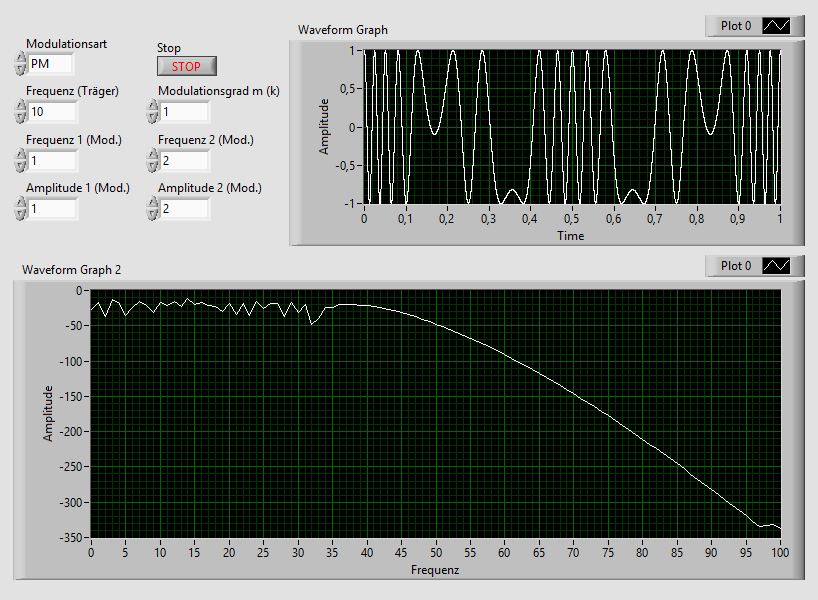
\includegraphics[width=0.7\textwidth]{pic/t10m1-2g1.png}
	\caption{Weiteres Beispiel zur Phasenmodulation. Die Parameter können der Abbildung entnommen werden.}
	\label{fig:a10}	
\end{figure} 
\begin{figure}[H]
	\centering
	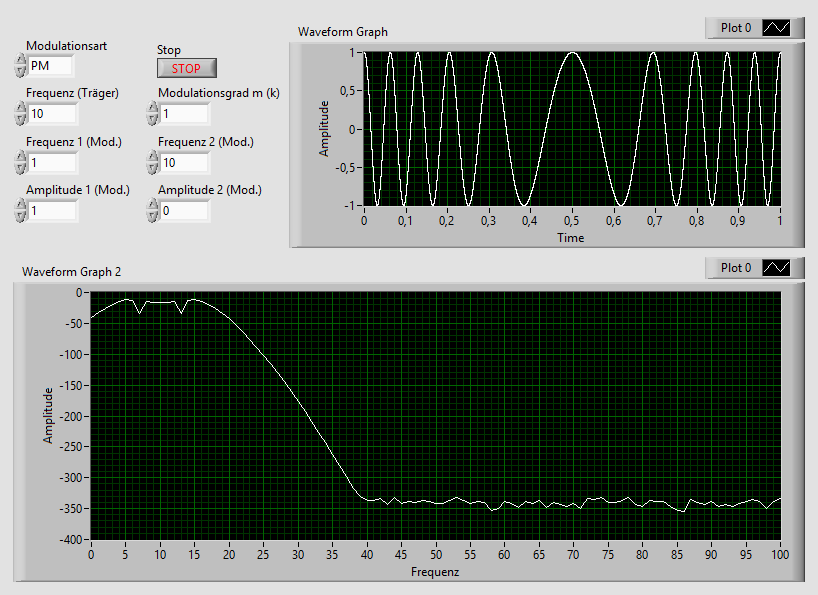
\includegraphics[width=0.7\textwidth]{pic/t10m1g1.png}
	\caption{Weiteres Beispiel zur Phasenmodulation. Die Parameter können der Abbildung entnommen werden.}
	\label{fig:a11}	
\end{figure} 

\newpage

\begin{figure}[H]
	\centering
	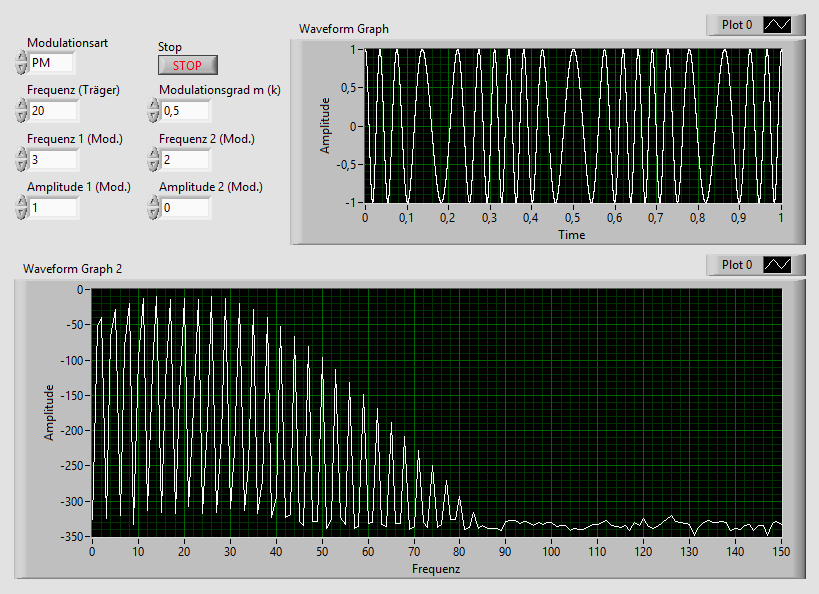
\includegraphics[width=1\textwidth]{pic/t20m3g05.png}
	\caption{Weiteres Beispiel zur Phasenmodulation. Die Parameter können der Abbildung entnommen werden.}
	\label{fig:a12}	
\end{figure} 
\subsection{Bilder zur Demodulation von Frequenz- und Phasenmodulierten Signalen}

\begin{figure}[H]
	\centering
	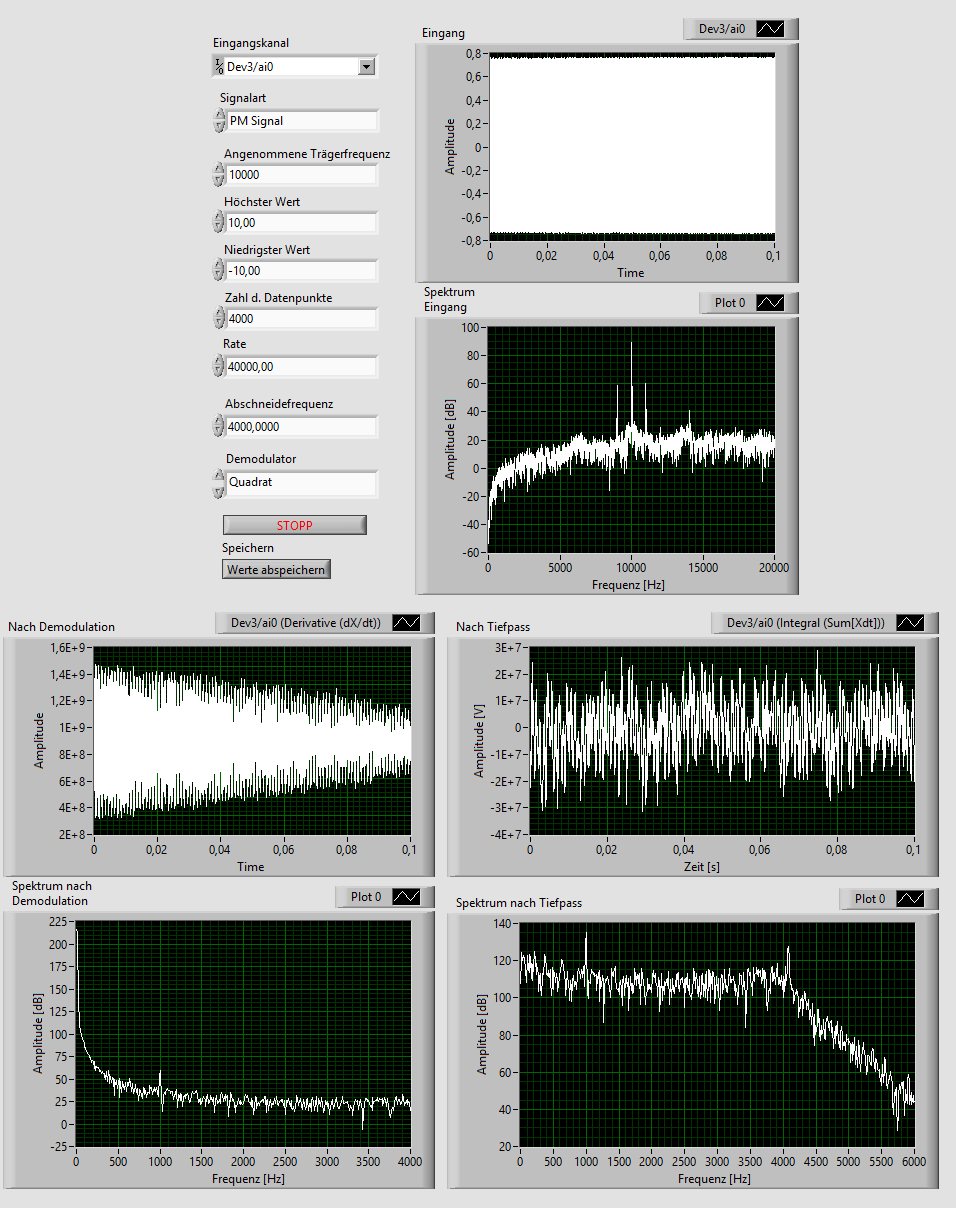
\includegraphics[width=0.8\textwidth]{pic/PM10k1k001.png}
	\caption{Weiteres Beispiel zur Demodulation eines Phasenmodulierten Signals. Die Parameter können der Abbildung entnommen werden.}
	\label{fig:a13}	
\end{figure} 

\begin{figure}[H]
	\centering
	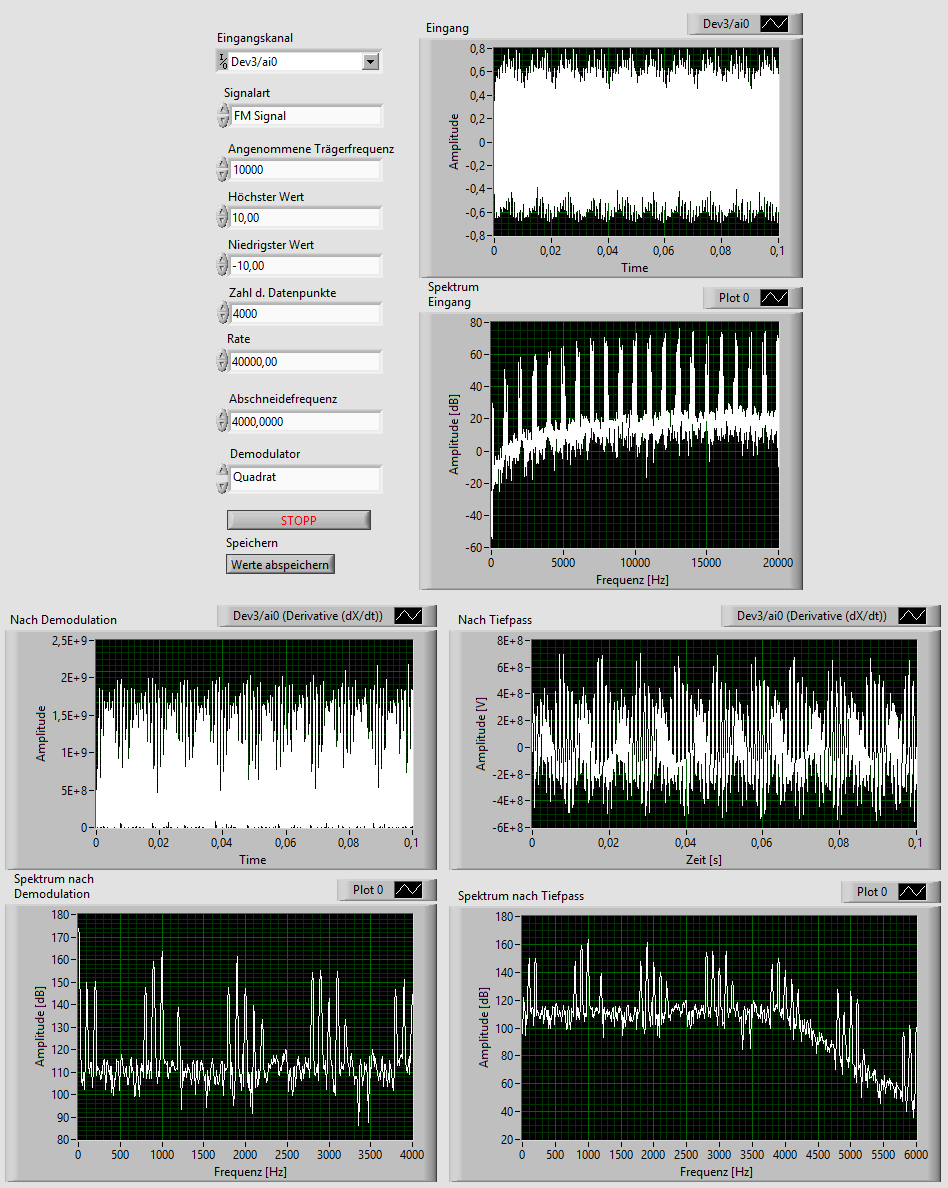
\includegraphics[width=1\textwidth]{pic/FM10k1k1.png}
	\caption{Weiteres Beispiel zur Demodulation eines Frequenzmodulierten Signals. Die Parameter können der Abbildung entnommen werden.}
	\label{fig:a14}	
\end{figure} 

\begin{figure}[H]
	\centering
	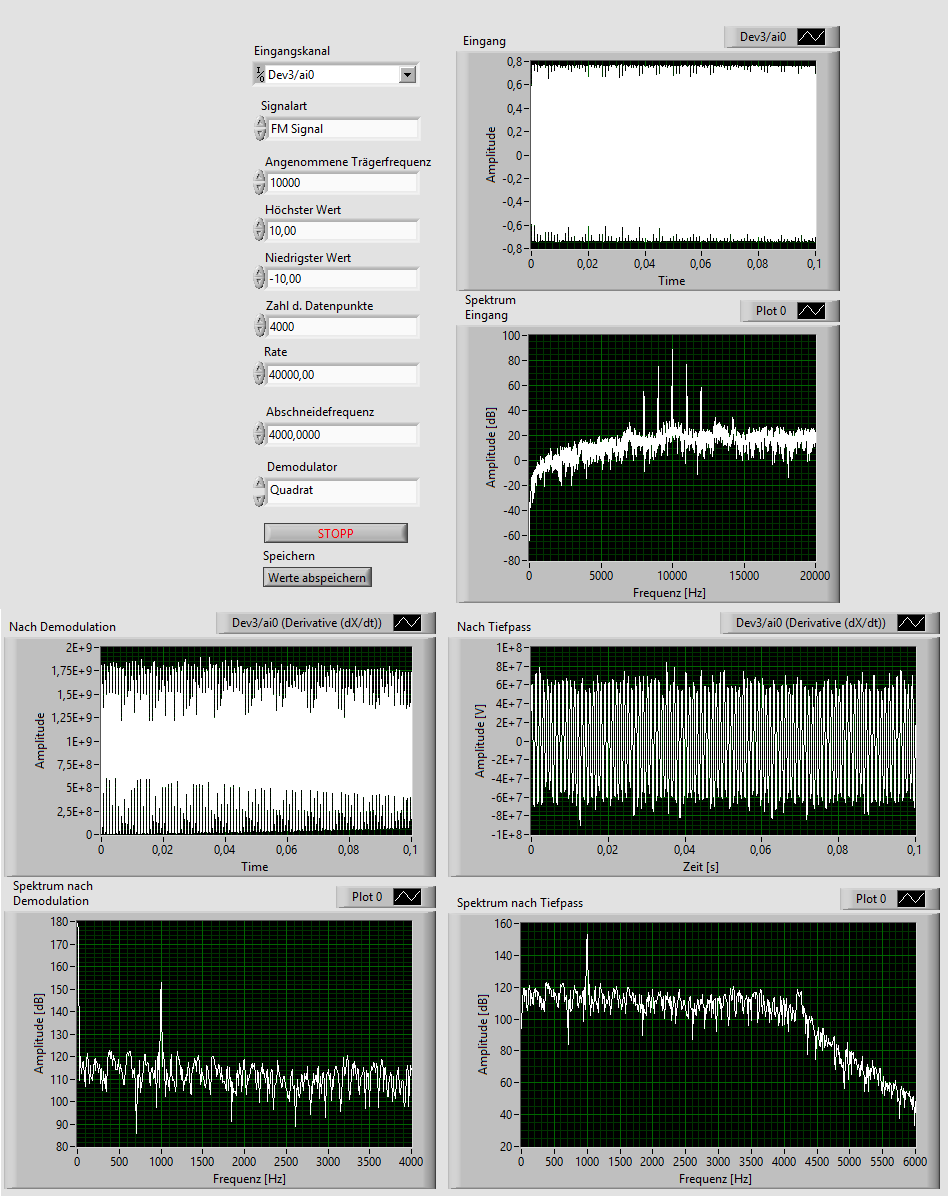
\includegraphics[width=1\textwidth]{pic/FM10k1k001.png}
	\caption{Weiteres Beispiel zur Frequenzmodulation. Die Parameter können der Abbildung entnommen werden.}
	\label{fig:a15}	
\end{figure} 

